\chapter{Modelling the System on MATLAB} \label{sec: MATLAB_Model}
    To aid in creating the first design, a mathematical model is required to determine the metrics of the system. This allows for rapid testing and optimization of parameters. 
    % For the full MATLAB code please see the online \href{https://github.com/Rayde29/24723061-Kruger-ProjectFile.git}{\textit{Project~File~here}}. 

    \section{Modelling the Rotor}
        To model the rotor, Blade Element Theory analysis was applied as described by \cite{blade_element_theory_2024}. The rotor was divided into segments and the lift and drag for each segment were calculated. This gives the profile of the thrust and torque along the rotor as can be seen in Figure~\ref{fig: thrust_over_radius} and Figure~\ref{fig: torque_over_radius}, respectively. The sum of each segment will result in the total thrust and torque produced by the rotor.
        The thrust and torque produced by each segment is an iterative process as the incoming flow velocity is unknown. In the first iteration, it is assumed to be zero, and thus the angle of attack is equal to the pitch of the rotor. The incoming air can be calculated using the first approximation of thrust and with Newton's First Law:
        \begin{align*}
            F & = ma\\
            T & = \frac{d(mV)}{dt}
        \end{align*}
        Assuming air above the rotor is stationary
        \begin{align*}
            T &= \dot{m}V\\
            T &= \rho V_{disk} A V
        \end{align*} 
        This gives the thrust in terms of the air velocity and velocity at the disk. As stated by momentum theory and by \cite{AflredAerodynamicsOfHelicopters}, the far wake velocity is half that of the air velocity \(V\) at the disk. Thus, for hover, assuming the free stream velocity is zero, the axial velocity at the disk can be given by

        \begin{align*}
            T &= (\rho \pi R^2 V_{disk} )2V_{disk}\\
            V_{disk} &= \sqrt{\frac{T}{2 \rho \pi R^2}}
        \end{align*}
        
        Using this and the angular rotation of the rotor, the angle of attack can be found as \[\alpha = \theta - \arctan\left(\frac{V_{disk}}{\frac{2}{3}R\omega_{Rotor}}\right)\] Two-thirds of the blade's length is used as the speed of the blade is not constant along its radius, so the speed of the centroid was used to try to approximate the average angle of attack along the blade. 
        It was seen that the thrust and torque converge after 25 iterations. Resulting in the profiles as seen in Figure~\ref{fig: thrust_over_radius} and Figure~\ref{fig: torque_over_radius}.


        \begin{figure}[h]
            \centering
            \begin{minipage}{0.45\textwidth}
                \centering
                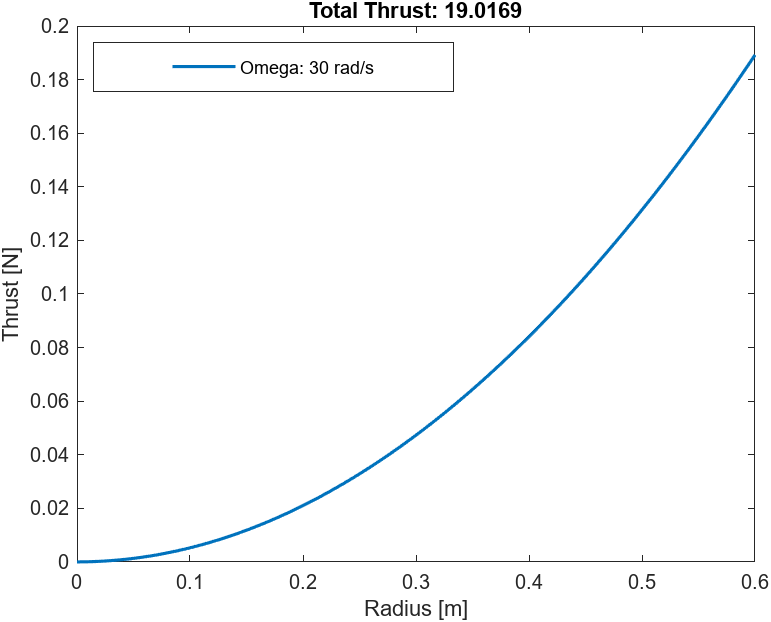
\includegraphics[width=\textwidth]{figs/Model/Rotor/Thrust_Vs_Radius.png}
                \caption{Thrust predicted over the length of the rotor}
                \label{fig: thrust_over_radius}
            \end{minipage}\hfill
            \begin{minipage}{0.45\textwidth}
                \centering
                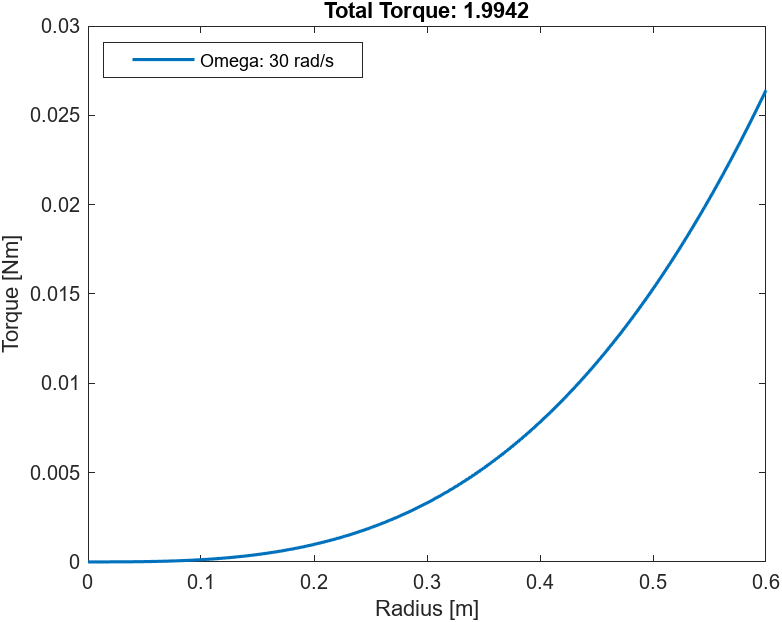
\includegraphics[width=\textwidth]{figs/Model/Rotor/Torque_Vs_Radius.png}
                \caption{Torque predicted over the length of the rotor}
                \label{fig: torque_over_radius}
            \end{minipage}
        \end{figure}

        % Using 300 segments resulted in predictions that are 0.5\% different from the value obtained using five thousand segments. This was an acceptable value and was used to reduce the computational cost of the model.

        % Using these results, the number of segments can be found which minimizes the computational cost, while having sufficient accuracy. Figure~\ref{fig: segments_vs_prediction} shows the predicted torque and thrust for the number of segments the rotor is split into. It can be seen that both graphs plateau and that after a certain amount of segments, the increase in accuracy is not beneficial for the computational power. The elbow of both of the predictions is around three hundred segments, which results in predictions that are 0.5\% different from the value obtained using five thousand segments. It was decided that it was sufficient accuracy for the computational cost and thus three hundred segments were used for the model.
        % \begin{figure}[h]
        %     \centering
        %     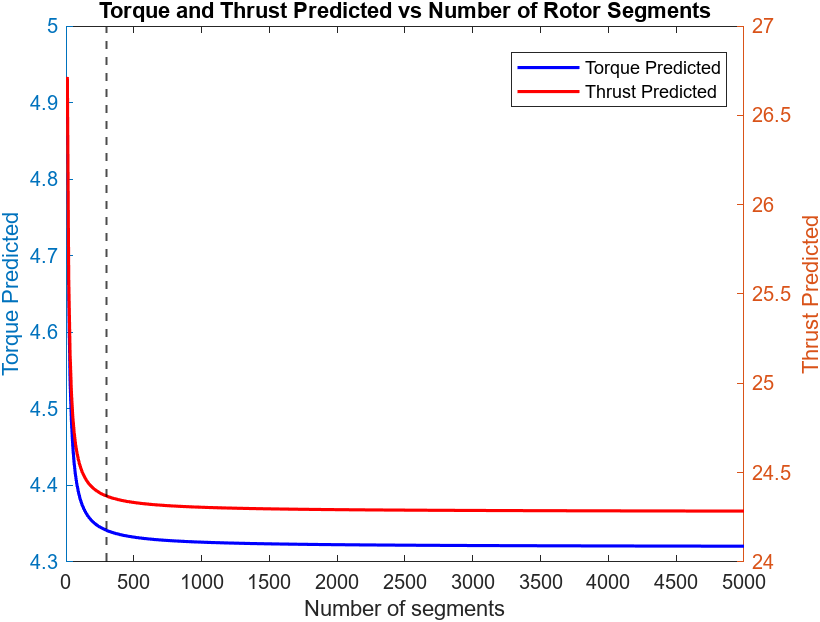
\includegraphics[width=0.6\textwidth]{figs/Model/Rotor/Segments_Vs_Error.png}
        %     \caption{Predicted torque and thrust vs the number of segments}
        %     \label{fig: segments_vs_prediction}
        % \end{figure}
        % \\
        The Blade Element analysis considers the 2D segments and thus does not take 3D effects into account. This results in the model underpredicting the torque and overpredicting the thrust produced. One of the assumptions neglects the tip vortices which will decreased the thrust produced. To compensate for the decreased thrust, the predicted thrust can be multiplied by a tip-loss factor \(b\). \cite{AflredAerodynamicsOfHelicopters} describe the tip-loss factor as a coefficient that is multiplied by the radius of the rotor for the thrust calculations. This assumes that from \(b\times R\) of the rotor, it will produce zero lift but still have drag. It is defined as 
            \begin{align}
                &b = 1 -\frac{\sqrt{2C_T}}{B}
            \end{align}
            \begin{minipage}{0.45\textwidth}
                \vspace*{-8mm}
                \begin{align*}
                    \text{where} \quad
                    &B  \text{ is the number of blades} \\
                    &C_T  \text{ is the rotor thrust coefficient}
                \end{align*}
                \end{minipage}
                \\
                
        The thrust coefficient is the thrust per unit blade span and can be defined as
        \begin{align}
            &C_T= \frac{T}{\pi R^2 \rho (\omega_{Rotor} R).^2}
        \end{align}
        \\
        The thrust and torque values were then calculated for a range of angular velocities and their values were stored. An exponential function is then fitted equations, as can be seen in Figure 2.3 and Figure 2.4, resulting
        in two equations that can be used to predict the total amount of thrust and torque produced for a given angular velocity, Eq. 2.3 and Eq. 2.4, respectively.
        \begin{align}
            T &= 0.01805 \omega_{Rotor} ^2 \label{eq: fitted_thrust}\\
            Q &= 0.002216 \omega_{Rotor} ^2 \label{eq: fitted_torque}
        \end{align}


        \begin{figure}[H]
            \centering
            \begin{minipage}{0.45\textwidth}
                \centering
                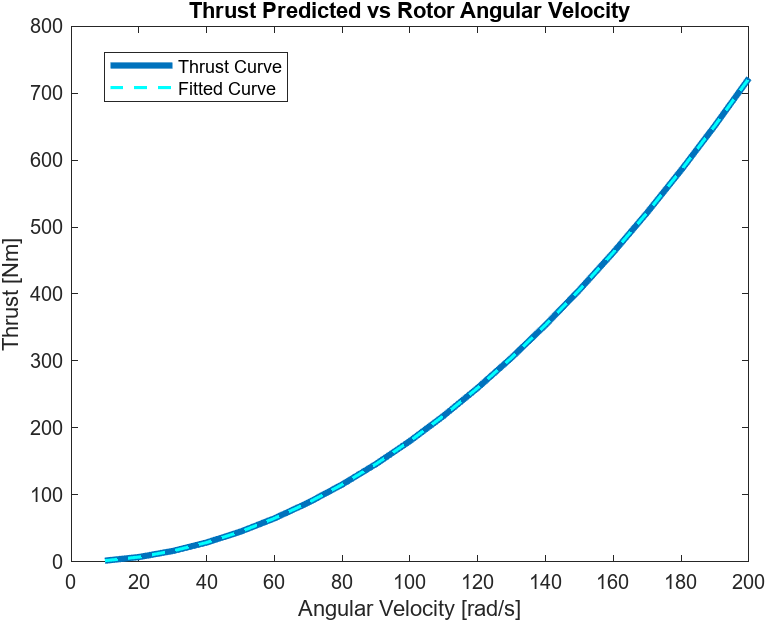
\includegraphics[width=0.8\textwidth]{figs/Model/Rotor/Thrust_Vs_Rotor_Angular_Velocity.png}
                \caption[Rotor thrust vs angular velocity]{Thrust predicted vs angular velocities and the fitted exponential equation}
                \label{fig: thrust_vs_angular_velocity}
            \end{minipage}\hfill
            \begin{minipage}{0.45\textwidth}
                \centering
                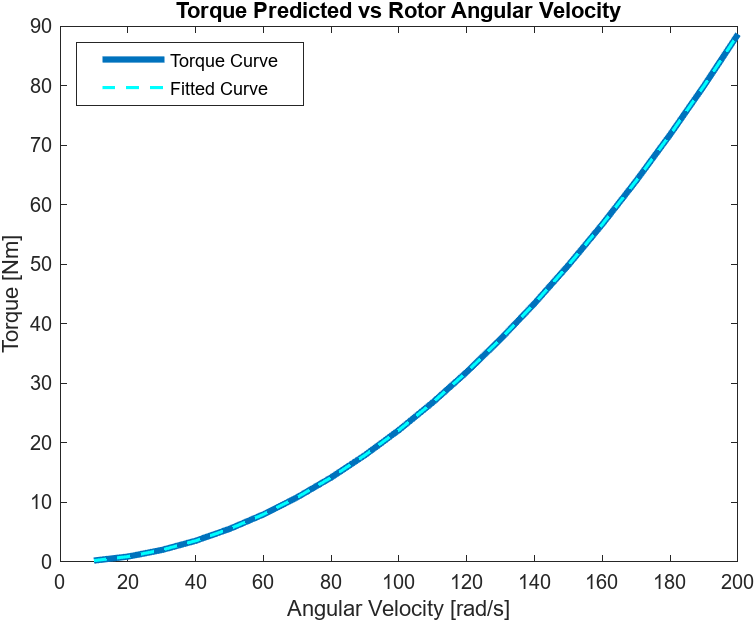
\includegraphics[width=0.8\textwidth]{figs/Model/Rotor/Torque_Vs_Rotor_Angular_Velocity.png}
                \caption[Rotor torque vs angular velocity]{Torque predicted vs angular velocities and the fitted exponential equation}
                \label{fig: torque_vs_angular_velocity}
            \end{minipage}
        \end{figure}
    \section{Modelling the Propellers}
        The thrust and torque produced by the propellers were calculated using one section with the radius being two-thirds of the blade length. The propeller’s pitch is described by the distance the propeller moves forward per rotation and thus to find the average angle of the pitch it can be found as\[\theta_{prop} = \arctan\left(\frac{\text{Pitch}}{\pi d}\right)\]
        The incoming airflow of each propeller can be found by multiplying the angular velocity of the rotor by the position along the rotor blade of the propellers. The high velocities of the inflowing air will decrease the angle of attack. This requires the propellers to have high angular velocities to ensure an angle of attack that produces thrust.
        \\
        As the incoming air velocity is dependent on the angular velocity, this results in a thrust and torque versus the angular velocity of the propellers to have a different shape depending on the angular velocity. This can be seen in  Figure~\ref{fig: prop_thrust_vs_velocity} and Figure~\ref{fig: prop_torque_vs_velocity}. 

        \begin{figure}[h]
            \centering
            \begin{minipage}{0.45\textwidth}
                \centering
                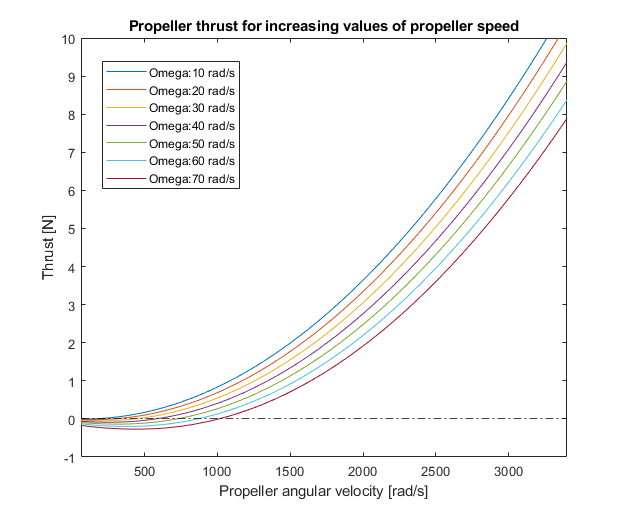
\includegraphics[width=\textwidth]{figs/Model/Props/Prop_thrust_vs_speed.png}
                \caption[Propeller thrust versus speed graph]{Propeller thrust versus its speed for different values of rotor angular velocity}
                \label{fig: prop_thrust_vs_velocity}
            \end{minipage}\hfill
            \begin{minipage}{0.45\textwidth}
                \centering
                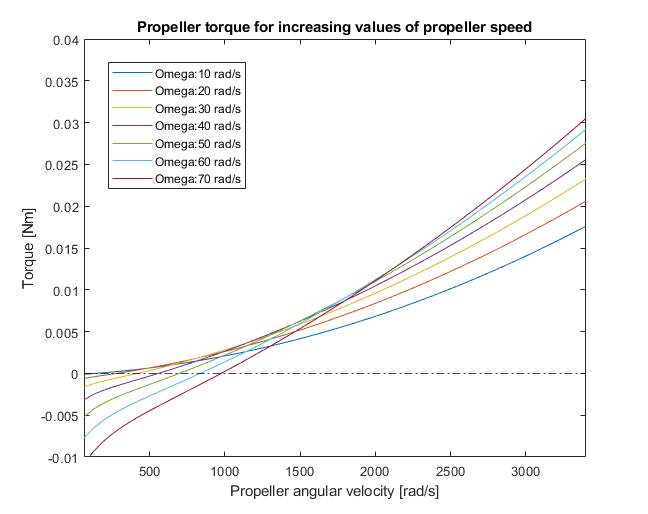
\includegraphics[width=\textwidth]{figs/Model/Props/Prop_torque_vs_speed.png}
                \caption[Propeller torque versus speed graph]{Propeller torque versus its speed for different values of rotor angular velocity}
                \label{fig: prop_torque_vs_velocity}
            \end{minipage}
        \end{figure}
        Each graph for the thrust, however, can be fitted by a parabolic graph, but with different coefficients depending on the rotor's angular velocity. The solution for this was to find a relationship between the coefficients and the rotor's angular velocity. The change of these coefficients can be seen in Figure~\ref{fig: p1_coefficient},\ref{fig: p2_coefficient} and \ref{fig: p3_coefficient}, in which \[T_{prop} = P_1\omega_{prop}^2 + P_2\omega_{prop} +P_3\] 
        
        \begin{figure}[h]
            \centering
            \begin{minipage}{0.31\textwidth}
                \centering
                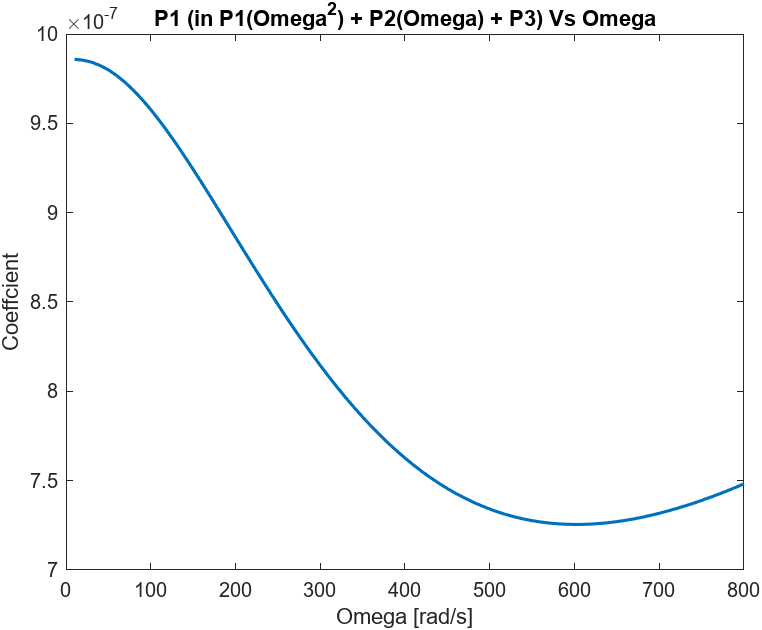
\includegraphics[width=\textwidth]{figs/Model/Props/P1_Coeffcient.png}
                \caption{Coefficient P1}
                \label{fig: p1_coefficient}
            \end{minipage}\hfill
            \begin{minipage}{0.31\textwidth}
                \centering
                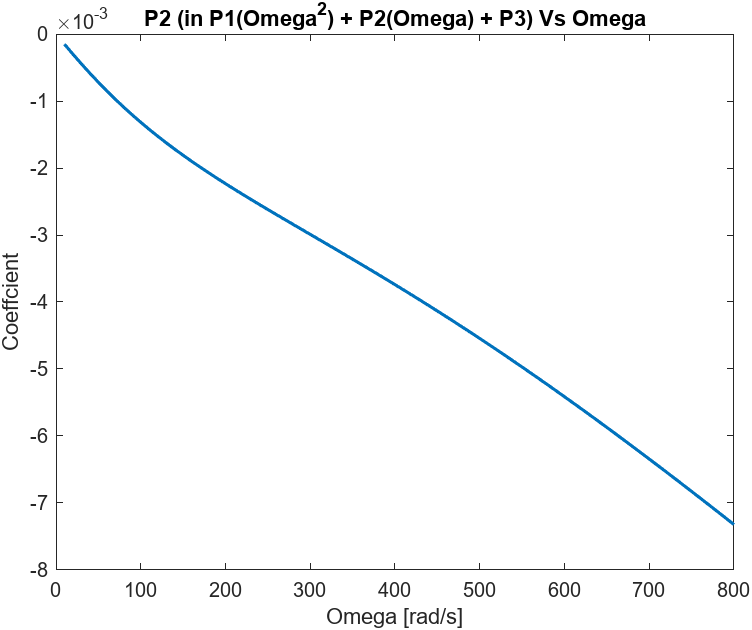
\includegraphics[width=\textwidth]{figs/Model/Props/P2_Coeffcient.png}
                \caption{Coefficient P2}
                \label{fig: p2_coefficient}
            \end{minipage}\hfill
            \begin{minipage}{0.32\textwidth}
                \centering
                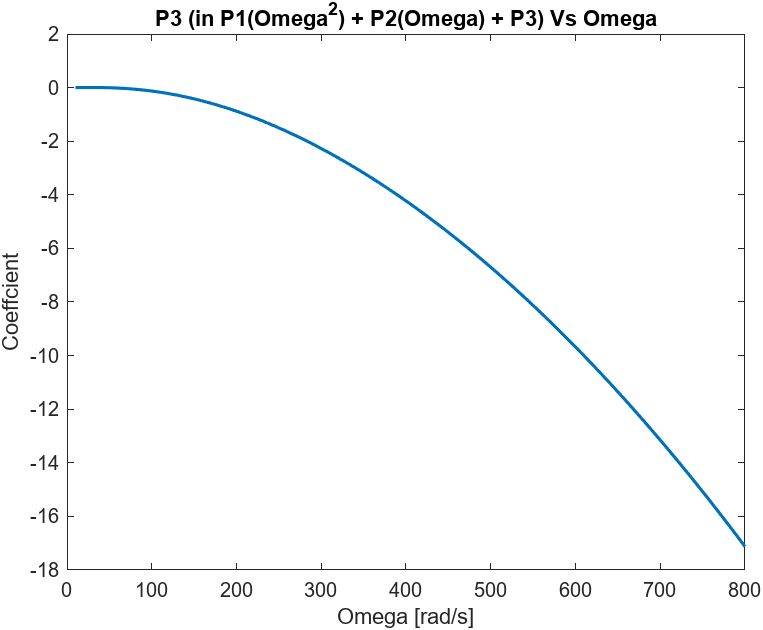
\includegraphics[width=0.99\textwidth]{figs/Model/Props/P3_Coeffcient.png}
                \caption{Coefficient P3}
                \label{fig: p3_coefficient}
            \end{minipage}
        \end{figure}
        From these graphs, clear relationships can be seen with all three coefficients and the angular velocity. Fitting curves to each coefficient result in the Eq.~\ref*{eq: prop_thrust}, which fully describes the thrust produced by tip-thrust.
        \begin{align}
            T_{prop}&=
            \left((-2.500\times 10^{-16})\omega_{rotor} ^3 + (1.517\times 10^{-12})\omega_{rotor} ^2 + (-1.314\times 10^{-9})\omega_{rotor} \right.\notag\\
            &\left. + (1.037\times 10^{-6})\right)\omega_{prop}^2 + \left((-7.806\times 10^{-12})\omega_{rotor}^2+(7.144\times 10^{-9})\omega_{rotor}^2 \right. \notag\\
            &\left. + (-1.301\times 10^{-5})\omega_{rotor}  -0.0003 \right)\omega_{prop}+\left( (-4.593\times 10^{-5})\omega_{rotor}^2 \right. \notag\\
            &\left.+ (-1.006\times 10^{-3})\omega_{rotor} +0.2227\right) \label{eq: prop_thrust}
        \end{align}

    \section{Optimization of Tip Thrust Positions}
        Having the propulsion at the end of the rotor will maximize the torque produced, however, it will have a higher incoming airflow and require higher rotation from the tip-thrust motors to produce thrust. The optimum point of the tip-thrust motors would be where the thrust required for the torque is minimized, and the thrust produced is maximized.\\
        To find the optimum point the rotor angular velocity and tip thrust angular were kept constant at an expected operating value. The thrust produced by the motors as well as the thrust that would be required to produce the torque were calculated for each percentage length along the rotor as seen in Figure~\ref{fig: thrust_req_vs_available}. This took the hub diameter into account, thus at 0\% of the rotor span (i.e. the base of the rotor), the torque does not tend to infinity.

        \begin{figure}[h]
            \centering
            \begin{minipage}{0.45\textwidth}
                \centering
                \includegraphics*[width = \textwidth]{figs/Model/Rotor/Thrust_avaliable_vs_required.png}
                \caption[Thrust available and required for tip-thrust positions]{Thrust available and the thrust required for a position along the rotor}
                \label{fig: thrust_req_vs_available}
            \end{minipage}\hfill
            \begin{minipage}{0.45\textwidth}
                \centering
                \includegraphics*[width =\textwidth]{figs/Model/Rotor/Optimisation_curve.png}
                \caption{Optimization curve}
                \label{fig: optimization_curve}
            \end{minipage}
        \end{figure} 
        The thrust required and thrust available were standardized, so they could be compared. The two standardized sets of values were subtracted from each other and the turning point of the resulting graph was used as the optimized position along the rotor. As can be seen in Figure~\ref{fig: optimization_curve}, this is around 32.5\% along the rotor blade. While this does vary slightly depending on the motor's angular velocity, at the expected velocity a position of 32.5\%  of the rotor is optimum and is close to the mean for the position that incorporates the range of motor speed.\\
  
        As the thrusts will no longer be placed on the tip of the rotors, it was believed that they should be referred to as TORB motors (Thrust On Rotor Blade) from this point forward. This was chosen to give a more accurate name to this method of creating rotational actuation.
    % \section{Combined Model}
    %     Using the models created above, the system can take the amount of thrust required and will output the torque produced and required thrust. 
    %     \begin{align}
    %         \omega_{rotor} =& \sqrt{55.4T_{rotor}}\\
    %         Q_{Rotor} =& 0.1228T_{rotor}
    %         % T_{prop} = P_1\omega_{prop}^2 + P_2\omega_{prop} +P_3
    %         % \omega_{prop} = \frac{-\left[(-7.806 \times 10^{-12})\omega_{rotor}^2 + (7.144 \times 10^{-9})\omega_{rotor} - 1.301 \times 10^{-5}\right] + \sqrt{\left[(-7.806 \times 10^{-12})\omega_{rotor}^2 + (7.144 \times 10^{-9})\omega_{rotor} - 1.301 \times 10^{-5}\right]^2 - 4 \left[(-2.500 \times 10^{-16})\omega_{rotor}^3 + (1.517 \times 10^{-12})\omega_{rotor}^2 + (-1.314 \times 10^{-9})\omega_{rotor} + 1.037 \times 10^{-6}\right] \left[(-4.593 \times 10^{-5})\omega_{rotor}^2 + (-1.006 \times 10^{-3})\omega_{rotor} + 0.2227 - T_{prop}\right]}}{2 \left[(-2.500 \times 10^{-16})\omega_{rotor}^3 + (1.517 \times 10^{-12})\omega_{rotor}^2 + (-1.314 \times 10^{-9})\omega_{rotor} + 1.037 \times 10^{-6}\right]}
    %                     % \quad \Rightarrow \omega_{prop} =& -\left((-1.775\times 10^{-15})\left(\sqrt{161.5T_{Rotor}}\right) ^3 + (3.676\times 10^{-12}) \right. \notag\\
    %         % &\left.\times\sqrt{161.5T_{Rotor}} ^2  + (-1.974\times 10^{-9})\sqrt{161.5T_{Rotor}}\notag  \right) \pm  \\ 
    %         % & \left[(-1.775\times 10^{-15})\left(\sqrt{161.5T_{Rotor}}\right) ^3 + (3.676\times 10^{-12})\right] \notag
    %     \end{align}


        % \todo[color=blue!10]{Do the whole formula}

        
        \section{Pitch Model}
            To estimate the amount of torque required to change the pitch of the rotor a rotational mass-spring-damper model was created. This models the system which assumes there will be natural damping, so no artificial damping will be introduced, and the system will be rotating on a low friction bushing, thus the effects of friction have been neglected. The model assumes a value for the moment of inertia based on a CAD model of the rotor. \\
            Two models have been created, one for a step input to achieve a fixed pitch change and a second one to achieve a varying pitch to create sinusoidal output which can be seen in Figure~\ref{fig: pitch_change}. This will create a differential amount of thrust that will induce forward movement. For these two models, the control of the steady state of the system was the objective, and thus the rise time and overshoot was a lower priority.
            \begin{figure}[h]
                \centering
                \begin{minipage}{0.45\textwidth}
                    \centering
                    \includegraphics*[width =0.9\textwidth]{figs/Model/Pitch/Pitch_variation.jpg}
                    \caption{Pitch change sinusoidally}
                    \label{fig: pitch_change}
                \end{minipage}\hfill
                \begin{minipage}{0.45\textwidth}
                    \centering
                    \includegraphics*[width = 0.5\textwidth]{figs/Model/Pitch/Free_body_diagram_spring.jpg}
                    \caption{Free body diagram of tip thrust }
                    \label{fig: free_body_diagram}
                \end{minipage}
            \end{figure} 
            % \subsection{Step Input}
            % From Figure~\ref{fig: free_body_diagram}, a differential equation can be derived for a step input to give Eq.~\ref*{eq: step_input_reponse}.
            % % \todo[color=green!20]{Put the proper zeta in}
            % \begin{align}
            %     \ddot{\theta} +2\omega_{n}\zeta\dot{\theta} + \omega _{n}^2 \theta &= \frac{M_{required}}{I_{airfoil}} \label{eq: step_input_reponse}
            % \end{align}
            % As no artificial damping will be added to the system, it was assumed to be an under-damped system and an arbitrary dampening coefficient has been used, and it is assumed it is starting where \(\theta\) and \(\dot{\theta}\) is zero. Using this information, the solution to Eq.~\ref{eq: step_input_reponse} given by Eq.~\ref{eq: step_input_reponse_solution}.
            % \begin{align}
            %     \theta(t) &= Ae^{-\zeta \omega_n t}\sin(\omega_d t +\phi) + \frac{M_{required}}{k} \label{eq: step_input_reponse_solution}
            % \end{align}
            % \begin{minipage}{0.45\textwidth}
            %     \vspace*{-4mm}
            %     \begin{align*}
            %         \text{where} \quad
            %         &A = \frac{-\frac{M_{required}}{k}}{\sin(\phi)} \\
            %         &M_{required} = \theta_{required}k\\
            %         &\theta_{required} \text{ is the desired pitch}
            %     \end{align*}
            %     \end{minipage}
            %     \\
            %     \begin{figure}[h]
            %         \centering
            %         \includegraphics*[width = 0.65\textwidth]{figs/Model/Pitch/System_response _for _step_input.png}
            %         \caption{System response to a step input}
            %         \label{fig: step_response}
            %     \end{figure}
            %     Figure~\ref{fig: step_response} shows the system response to an applied moment that results in a steady state of 0.0873 rads (5\(^\circ\)). It can be seen that the response from the system has some oscillation, however its settling time is reasonably fast and would suffice for the proof of concept.
            %     \vspace{-5mm}
            \subsection{Sinusoidal Input}
                For a sinusoidal input the differential equation is given by Eq.~\ref*{eq: cos_input_reponse}
                \begin{align}
                    \ddot{\theta} +2\omega_{n}\zeta\dot{\theta} + \omega _{n}^2 \theta &= \frac{M_{required}}{I_{airfoil}}\cos(\omega_{rotor} t) \label{eq: cos_input_reponse}
                \end{align}
                % The same dampening coefficient which was used for the step input was used for the sinusoidal input. 
                As no artificial damping will be added to the system, it was assumed to be an under-damped system and an arbitrary dampening coefficient has been used, and it is assumed it is starting where \(\theta\) and \(\dot{\theta}\) is zero. This differential equation can be solved by Eq.~\ref{eq: cos_input_reponse_solution}
                \begin{align}
                    \omega(t) &= Ae^{-\zeta \omega_{n} t}\sin(\omega_d t + \phi) + X\cos (\omega_{rotor} - \beta) \label{eq: cos_input_reponse_solution}
                \end{align}
                \vspace*{-2mm}
                To find the torque required for a given steady state, first \(X\) must be determined. It can be seen that the exponential term will tend to zero as time tends to infinity, thus \(X = \theta_{required}\). Knowing this, the moment can be given by \[M_{required} = XI_{airfoil} \sqrt{\left(\omega_{n}^2 - \omega_{rotor}^2\right)^2 + \left(2 \zeta \omega_{n} \omega_{rotor}\right)^2}\] This produces the graph as seen in Figure~\ref{fig: cos_response}.
                \begin{figure}
                    \centering
                    \includegraphics*[width = 0.65\textwidth]{figs/Model/Pitch/System_response _for _sinusoidal_input.png}
                    \caption{System response to a sinusoidal input}
                    \label{fig: cos_response}
                \end{figure}
                The optimum spring stifness and damping coefficient that minimize the required torque were found be varying these two paramters and plotting it versus the resulting torque, shown in Figure~\ref{fig: 3d_plot}. Most notible was to minimize the torque required to change the pitch, the spring stiffness should be chosen such that the natural frequency of the system is clsoe to the rotor's angular velocity.
                % To find the optimum spring stiffness and damping coefficient which will produces the smallest required torque, these two parameters were changed, and the torque required was plotted vs these parameters resulting in the graph as shown in Figure~\ref{fig: 3d_plot}. With reference to the damping coefficient, it shows that the lower the coefficient, the lower the torque, however, this will affect how much the system's natural frequency influences the output. For the spring constant, it should be noted that there is a value for which the torque is minimized. After further inspection, it can be seen that choosing a spring constant which results in the natural frequency being close to \(\omega_{rotor}\) will require the lowest amount of torque to control.
                \begin{figure}[H]
                    \centering
                    \includegraphics*[width = 0.4\textwidth]{figs/Model/Pitch/Torque_stiffness_damping_surface.png}
                    \caption[Torque surface graph]{Surface graph showing of torque versus damping coefficient and spring stiffness}
                    \label{fig: 3d_plot}
                \end{figure}
        % T_{prop}&=
        % \left((-1.775\times 10^{-15})\omega_{Rotor} ^3 + (3.676\times 10^{-12})\omega_{Rotor} ^2  \right.\notag\\
        % &\left. + (-1.974\times 10^{-9})\omega_{Rotor} + (1.050\times 10^{-6})\right)\omega_{prop}^2 + \left((-3.093\times 10^{-12})\right. \notag\\
        % &\left. \times \omega_{Rotor}^2 +(-7.582\times 10^{-10})\omega_{Rotor}^2  (-1.391\times 10^{-5})\omega_{Rotor}  -0.0005 \right)\omega_{prop} \notag\\
        % & \left( (-7.745\times 10^{-5})\omega_{Rotor}^2 + (-1.935\times 10^{-3})\omega_{Rotor} +0.2796\right) \label{eq: prop_thrust}
